\documentclass[a4paper, 11pt]{article}
\usepackage{geometry}
\geometry{letterpaper, margin=1in}
\usepackage{amsmath}
\usepackage{amssymb}  
\usepackage{amsthm}
\usepackage{ulem} 
\usepackage{graphicx}
\usepackage{enumitem} % use for making lettered list 
\usepackage{bbm} % use for making the 1 identity operator EX: \mathbbm{1}
\usepackage{subfig} 
\graphicspath{ {images/} }

% format to allow bolded theorems, corollaries, etc... 
\newtheorem*{theorem}{Theorem}
\newtheorem*{corollary}{Corollary}
\newtheorem*{lemma}{Lemma}
\newtheorem*{definition}{Definition}
\newtheorem*{Example}{Example} 
\newtheorem*{Remark}{Remark}

% stop typing \mathbb a thousand times 
\newcommand{\R}{\mathbb{R}}
\newcommand{\C}{\mathbb{C}}
\newcommand{\F}{\mathbb{F}}
\newcommand{\Mat}[2]{\mathcal{M}_{#1\times#2}}

% change margins for solution
\newenvironment{solution}{%
	\begin{list}{}{%
			\setlength{\topsep}{0pt}%
			\setlength{\leftmargin}{1.5cm}%
			\setlength{\rightmargin}{1.5cm}%
			\setlength{\listparindent}{\parindent}%
			\setlength{\itemindent}{\parindent}%
			\setlength{\parsep}{\parskip}%
		}%
		\item[]}{\end{list}}

\begin{document}
%Header-Make sure you update this information!!!!
\noindent
\large\textbf{Homework 2} \hfill \textbf{John Waczak} \\
\normalsize MTH 443 \hfill  Date: \today \\
Dr. Schmidt \hfill Worked with: Garrett Jepson 
\par\noindent\rule{\textwidth}{0.4pt} \\

\noindent(1). (a) Clearly state under what conditions the range and null space of a linear transformation T are the same set. 
	\begin{solution}
		\noindent Consider a general linear transformation $T:V\to W$ where $V$ and $W$ are $\F$-vector spaces. In order for the range of T to be equal to its null space, we must have the following
			\begin{enumerate}
				\item $W = V$ 
				\item $\dim(V)$ is even 
				\item $\operatorname{rank}(T) = \operatorname{nullity}(T)$
			\end{enumerate}
	\end{solution}

\noindent(b) Prove your assertion 
	\begin{solution}
		\begin{proof} 
			\noindent Consider a linear transformation $T:V\to W$ for $V,W$ $\F$-vector spaces. Our goal is to show that the above conditions are satisfactory requirements for the range to be equal to the null space of T. First, in order for these to be the same set we must have $V=W$. If we do not, then even if the two supspaces are isomorphic we will not have that they are the \textit{same set}. \\ 
		
			Next, recall from class that the rank nullity theorem (2.3) asserts 
				\begin{equation*}
					\operatorname{rank}(T) + \operatorname{nullity}(T) = \dim(V) 
				\end{equation*}
			Also, further recall from Theorem 2.1 that $\ker(T)$ and $T(V)$ are subspaces of V and W. Therefore given a set of vectors $\{v_i\}$ is in either of the spaces, $\operatorname{span}(\{v_i\})$ must also be in these spaces. If the $\dim(V)$ is not even, then by the above theorem it must be true that $\operatorname{rank}(T)\neq\operatorname{nullity}(T)$. As these quantities refer to the dimenions of the range and null space then the number of vectors needed to span the range is not equal to the number of vectors needed to span the null space. This implies that $T(V)\neq \ker(T)$. Therefore, we must have that $\dim(V)$ is even. \\ 

			We now consider requirement 3. If requirements 1 and 2 hold and $\dim(V)=2$, we have that $\operatorname{rank}(T)=\operatorname{nullity}(T)$. If $\dim(V)\geq 2$ and $\dim(V)$ is even then it may be that $\operatorname{rank}(T) = k$ and $\operatorname{nullity}(T)= m$ where $k+m = \dim(V)$ but $k\neq m$. If this is true then by the same argument as before a different number of vectors will span  each space and so they can not be the same set (consider the difference between a 3-space and a line in 3-space). Therefore, we must also have that $\operatorname{rank}(T) = \operatorname{nullity}(T)$. \\ 
			
			Given these requirements, both the $\operatorname{rank}(T)$ and $\operatorname{nullity}(T)$ will be the same and so the range and kernel will lie in the same vector space and have the same number of basis vectors. Because every vector space contains the span of its basis, this implies that the range and the kernel will have the same span. Thus, given 1, 2, and 3, we have that the range and kernel are the same set. 
			
		\end{proof} 
	\end{solution} 
\noindent(c) Give an example
	\begin{solution}
		\noindent\textbf{Example:} Consider the linear transformation $T:\F^2\to\F^2$ given by
			\begin{equation*}
				T(x,y) = (0, x) 
			\end{equation*}
		Acting this transformation on the canonical basis vectors $e_1, e_2$ generates the matrix representation for $T$ denoted $A_T \in \mathcal{M}_{2\times2}$. 
			\begin{equation*}
				A_T = \begin{pmatrix}
					0 & 0 \\ 
					1 & 0 
				\end{pmatrix}
			\end{equation*}
		Then solutions to the equation $Ax=0$ are easily shown by row operations to be of the form
			\begin{equation*}
				\begin{pmatrix} 0 \\ \lambda \end{pmatrix}, \quad \forall \lambda\in\F
			\end{equation*}
		Therefore the null space of this linear transformation is
			\begin{equation*}
				\ker(T) = \{(x,y)\in \F^2| T(x,y) = (0,0)\} = \operatorname{span}(e_2)
			\end{equation*}
		Now, the range of this transformation, $T(\F^2)$ is defined as 
			\begin{equation*} 
				T(\F^2) = \{w\in \F^2 :\; \exists v \in \F^2 \text{ with } T(v)=w\}
			\end{equation*}
		Thus, from our matrix we can see that $\forall$ $v=(x,y)^t \in \F^2$ we have the following
			\begin{align*}
				Av &= \begin{pmatrix}0 & 0 \\ 1 & 0\end{pmatrix}\begin{pmatrix}x \\ y\end{pmatrix}\\ 
				&= \begin{pmatrix}0 \\ x\end{pmatrix}
			\end{align*}
		As $(x,y)$ was arbitrary, we see that the range is also given by 
			\begin{equation*} 
				T(\F^2) = \operatorname{span}(e_2)
			\end{equation*}
		From this we conclude that T is an example of a linear transformation with a range equal to its null space. \\ 
	\end{solution}

\noindent(2). Let V and W be finite dimensional vector spaces, and suppose that U is a vector subspace of V. Prove that there exists a surjective linear transformation from V to W whose null space is U if and only if $dim(U) = dim(V) - dim(W)$. \\
	\begin{solution}
		\begin{proof}
			$(\rightarrow)$ Assume $T:V\to W$ is a surjection with $\ker(T)=U\subseteq V$. By the definition of surjective we have that $\forall w\in W$ $\exists v \in V$ such that $T(v) = w$. In other words, 
				\begin{equation*}
					T(V) = W 
				\end{equation*}
			by the rank nullity theorem, we have that 
				\begin{align*}
					\dim(V) &= \dim(T(V)) + \dim(\ker(T)) \\ 
						&= \dim(T(V)) + \dim(U) \quad \text{ by hypothesis} \\ 
						&= \dim(W) + \dim(U) \quad \text{ by surjection of T} \\ 
					\Rightarrow \dim(U) &= \dim(V) - \dim(W) 
				\end{align*}
			$(\leftarrow)$ Let $U\subseteq V$ be a subspace such that $\dim(U)=\dim(V)-\dim(W)$. Assume for contradiction that $\forall T:V\to W$ where $T$ is a surjection, $\ker(T)\neq U$. Since $T$ is a surjection, we have that
				\begin{equation*}
					T(V) = W \Rightarrow \dim(T(V)) = \dim(W) 
				\end{equation*}
			By rank nullity theorem, we have that
				\begin{align*}
					\dim(V) &= \dim(T(V)) + \dim(\ker(T)) \\ 
						&= \dim(W) + \dim(\ker(T))  \\
					\Rightarrow \dim(W)+\dim(U) &= \dim(W) + \dim(\ker(T)) \\
					\Rightarrow \dim(U) &= \dim(\ker(T)) 
				\end{align*}
			but we know that $U\neq \ker(T)$ by our hypothesis. Since $\ker(T)$ and $U$ are subspaces they must contain the span of their basis vectors. The dimension is the number of vectors in a basis so from the above it must be true that 
				\begin{equation*}
					U   = \ker(T)  
				\end{equation*}
			This contradicts our hypothesis. Therefore we have that if $U\subseteq V$ such that $\dim(U) = \dim(V)-\dim(W)$ then there exists a surjection $T:V\to W$ such that $\ker(T) = U$. This completes the proof. 
		\end{proof}
	\end{solution}

\noindent(3). Let $T:\R^3\to \R^2$ and $U:\R^2\to \R^3$ be linear transformations. What is the rank of $UT$? (That is, list all the possibilities and prove your list is complete and correct)\\
	\begin{solution}
		\begin{proof}
		\noindent Let's examine $T$ individually. Recall that the image of a transformation is a subspace of the codomain. Therefore, $T(\R^3)\subseteq \R^2$. This means that $T(\R^3)$ may have at most 2 basis vectors... i.e. $T$ has rank at most 2. The relationships between these transformations are captured in the following diagram.
		
			\begin{figure}[!hbt]
				\centering
				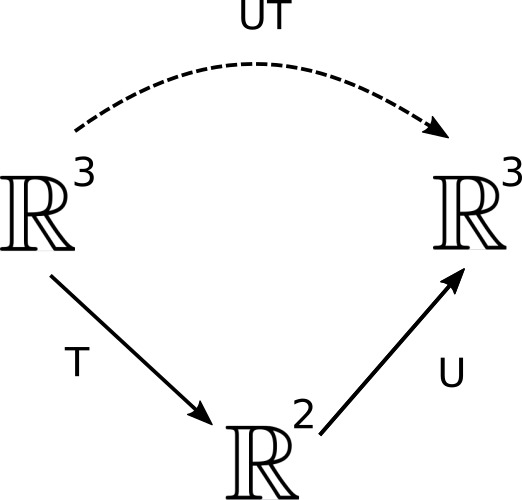
\includegraphics[width=0.25\columnwidth]{compositionDiagram}
			\end{figure}
		
		\noindent Now recall that for a general linear transformation $L:V \to W$ the rank nullity theorem guarantees that $\dim(L(V))\leq \dim(V)$. Therefore by chaining this together we see that
			\begin{align*}
				\operatorname{rank}(UT) &= \dim(UT(\R^3)) \\ 
					&= \dim U(T(\R^3)) \leq \dim(T(\R^3) \leq 2
			\end{align*}
		Now let's make sure that the $\operatorname{rank}(UT)$ can, in fact, be zero. Let U be the zero transformation, i.e. $U:\R^2\to\R^3$ s.t. $(x,y)\mapsto(0,0,0)$. Then the composition with T is $UT:\R^3\to\R^3$ s.t. $(x,y,z)\mapsto(0,0,0)$. Because every vector is sent to the zero vector, the nullity of this transformation must be the dimension of the domain i.e. 3. Then then by the rank nullity theorem, the rank of $UT$ is zero. \\
		
		\noindent Therefore we conclude that the only possible values for the rank of $UT$ are
			\begin{equation*}
				\operatorname{rank}(UT) \in \{0, 1, 2\} 
			\end{equation*}
		\end{proof}
	\end{solution}

\noindent(4). Given $T:V\to V$ is a linear transformation and W a subspace of V, we say W is T-invariant if $Tw \in W$ for all $w \in W$. \\

\noindent(a). Prove that the range and null space are T-invariant. \\
	\begin{solution}
		\begin{proof}
			\noindent Consider a $v_2\in T(V)\subseteq V$. Then $\exists v_1 \in V$ such that $v_2 = T(v_1)$. Now since T maps V to itself then $\exists v_3 \in V$ such that $v_3 = T(v_2)$ thus the range of T is T-invariant. \\ 
			
			\noindent Recall that $\ker(T) = \{v\in V | T(v) = 0_V\}$. Then if $v\in\ker(T)$ we have that $T(v) = 0$. Since $T(0)=0$ for any linear transformation then $0\in\ker(T)$. Thus $\ker(T)$ is T-invariant. \\
		\end{proof}
	\end{solution}

\noindent(b)Suppose that W is a k-dimensional T-invariant subspace of V. Show that there is a basis $\mathcal{B}$ of V such that $[T]_\mathcal{B}$ has the form $\begin{pmatrix}
A & B \\ O & D
\end{pmatrix}$ where $A\in\mathcal{M}_{k\times k}$ and $O$ is the $(n-k)\times k$ zero matrix. \\
	\begin{solution}
		\begin{proof}
			\noindent Let V be a vector space of dimension $n$ and W a T-invariant subspace of V with dimension $k$. Consider a basis for W $\mathcal{B}_W = \{w_1,...,w_k\}$. Extend this basis to a basis via the replacement theorem to a basis for $V$ such that $\mathcal{B}= \{w_1,...,w_k, v_1,..., v_\ell\}$ where $k+\ell = n$. \\ 
			
			\noindent As W is a T-invariant subspace of V, we have $T(W)\subseteq W$. From this it follows that every vector in W may be written as a linear combination of the basis vectors $\mathcal{B}_w$ alone. Thus,
				\begin{align*}
					T(w_1) &= \sum_i^k a_{1i} w_i + \sum_i^\ell 0v_i \\ 
					T(w_2) &= \sum_i^k a_{2i} w_i + \sum_i^\ell 0v_i \\ 
					\vdots \qquad	& \qquad \vdots  \qquad \qquad \quad \vdots \\ 
					T(w_k) &= \sum_i^k a_{ki} w_i + \sum_i^\ell 0v_i 
				\end{align*}
			Then for the rest of the basis vectors $\{v_1, ... ,v_\ell\}$ we will have some other linear combinations which we will denote with b's and d's 
				\begin{align*}
					T(v_1) &= \sum_i^k b_{1i} w_i + \sum_i^\ell d_{1i}v_i \\ 
					T(v_2) &= \sum_i^k b_{2i} w_i + \sum_i^\ell d_{2i}v_i \\ 
					\vdots \qquad	& \qquad \vdots  \qquad \qquad \quad \vdots \\ 
					T(v_\ell) &= \sum_i^k b_{ki} w_i + \sum_i^\ell d_{\ell i}v_i 
				\end{align*}
			Now the matrix representation for a linear transformation is determined by writing $T(\beta_j)$ as a column for each basis vector $\beta_j$. Thus the matrix for this transformation is given by 
				\begin{align*}
					[T]_\mathcal{B} &= \begin{pmatrix}
						a_{11} & a_{12} & \cdots & a_{1k} & b_{11} & b_{12} & \cdots & b_{1\ell} \\ 
						a_{21} & a_{22} & \cdots & a_{2k} & b_{21} & b_{22} & \cdots & b_{2\ell} \\ 
						\vdots & \vdots & \vdots & \vdots & \vdots & \vdots & \vdots & \vdots \\ 
						a_{k1} & a_{k2} & \cdots & a_{kk} & b_{21} & b_{k2} & \cdots & b_{k\ell} \\
						0	   & 0		& \cdots & 0 	  & c_{11} & c_{12} & \cdots & c_{1\ell} \\
						0	   & 0		& \cdots & 0 	  & c_{21} & c_{22} & \cdots & c_{2\ell} \\
						\vdots & \vdots & \vdots & \vdots & \vdots & \vdots & \vdots & \vdots \\ 
						0	   & 0		& \cdots & 0 	  & c_{\ell1} & c_{\ell2} & \cdots & c_{\ell\ell} \\
					\end{pmatrix} \\ 
					& \\ 
					&= \begin{pmatrix}
						A & B \\ 
						O & D 
					\end{pmatrix}
				\end{align*}
			Where $A$ is a $k\times k$ matrix and O is the $(n-k)\times k$ zero matrix. 
		\end{proof}
	\end{solution}

\end{document} 


























